%!TEX root = ../username.tex
\chapter{YOLO Variation} \label{chap:yolo_variation}

In addition to the Region-based Convolutional Neural Network (R-CNN) family, the other model family we will discuss in this section is You Only Look Once (YOLO). Similar to the R-CNN family, the YOLO family is also designed to perform object detection and can be expanded to other tasks like instance segmentation or semantic segmentation. However, unlike the R-CNN family, the model in the YOLO family frames the object detection task as a single-stage regression problem instead of a double-stage regression problem \cite{yolov3_2018}. 

The models in the R-CNN family are considered as double-stage methods because the model generates a region of interest (RoI) and classifies each RoI using two different algorithms or networks. That is, while RoI generation can be done with a greedy algorithm (like Selective Search) or a fully connected convolutional network (like RPN), the model uses another CNN for feature extraction (like AlexNet, VGG16, and ResNet) and adapt it to perform classification for each generated RoI \cite{Girshick_R_CNN_2013, fast_rcnn_og, faster_rcnn_2015}. For this reason, the object detection task is separated into two tasks: localization task and classification task, where each task is completed by a different network.

On the other hand, the models in the YOLO family is utilized a single convolution neural network to simultaneously predict both the bounding box and the classification label for each object in the input image \cite{yolov1_2016}. Therefore YOLO model family is designed to only evaluate an image once with a single CNN for the object detection task. Hence the name You Only Look Once. In this chapter, we will discuss different versions of the YOLO model.

\section{YOLOv1}  \label{sec:yolov1}

The first YOLO model was proposed in the "You Only Look Once: Unified, Real-Time Object Detection" paper in 2015 \cite{yolov1_2016}. Since there will be improvement version of the model, we denote this first model is YOLOv1, which is widely accepted in the computer vision research community \cite{understand_cnn_vs_yolo}. The YOLOv1 is designed to be a realtime object detection model. The YOLOv1 model is a three steps process, as shown in Firgure \ref{fig:yolov1_process}. In the first step, the model take an image of any size as input and resize the image to the fix size of $448 \times 448$. In the second step, the model predict mutiple bounding box, each with a objectiveness confidence score, and multiple classification for each detected object. Since the model predict multiple bounding box and classfication for each detected object, a non-maximum suppression (NMS) algorithm, as described in Subsection \ref{subsec:rpn}, is applied to assign one bounding box and one classification label per predicted object in the last step.

\begin{figure}[!ht]
    \centering
    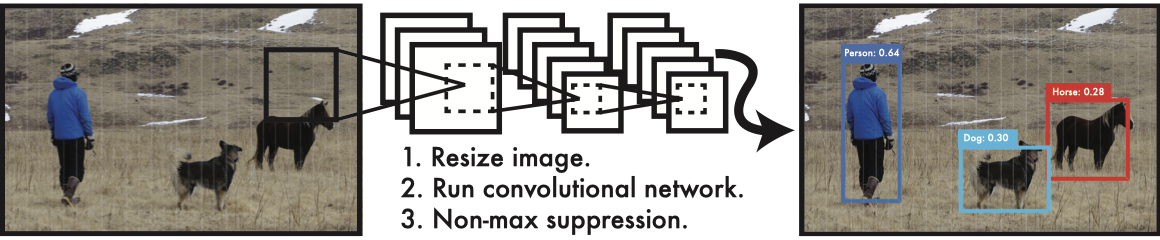
\includegraphics[width=4in]{figures/yolov1_process.png}
    \caption{YOLOv1 object detection process \cite{yolov1_2016}} 
    \label{fig:yolov1_process}
\end{figure}

In the original paper, the authors claim that YOLOv1 model have three main benifit \cite{yolov1_2016}. First, YOLOv1 is extremely fast, processing 45 images per second compare to 7 images per second achieved by the Faster R-CNN model with VGG16 backbone. However, this is achieved at the cost of 9.8\% reduction in mean average precision (mAP) score, i.e., 63.4\% and 73.2\% for mAP score of YOLOv1 and Faster R-CNN, respectively. The second benifit is YOLOv1 learn a general representation of object, thus it tend to perform better compare to R-CNN based model when predicting for other domain like artwork. The third benifit it it see the entire image during bounding box regression and classification compare to R-CNN classifier and bounding box regressor only see the ROI. This change allow YOLOv1 to encodes contextual information about classes and thus reduce the number of false positive.

\subsection{Network Architecture}

\begin{figure}[!ht]
    \centering
    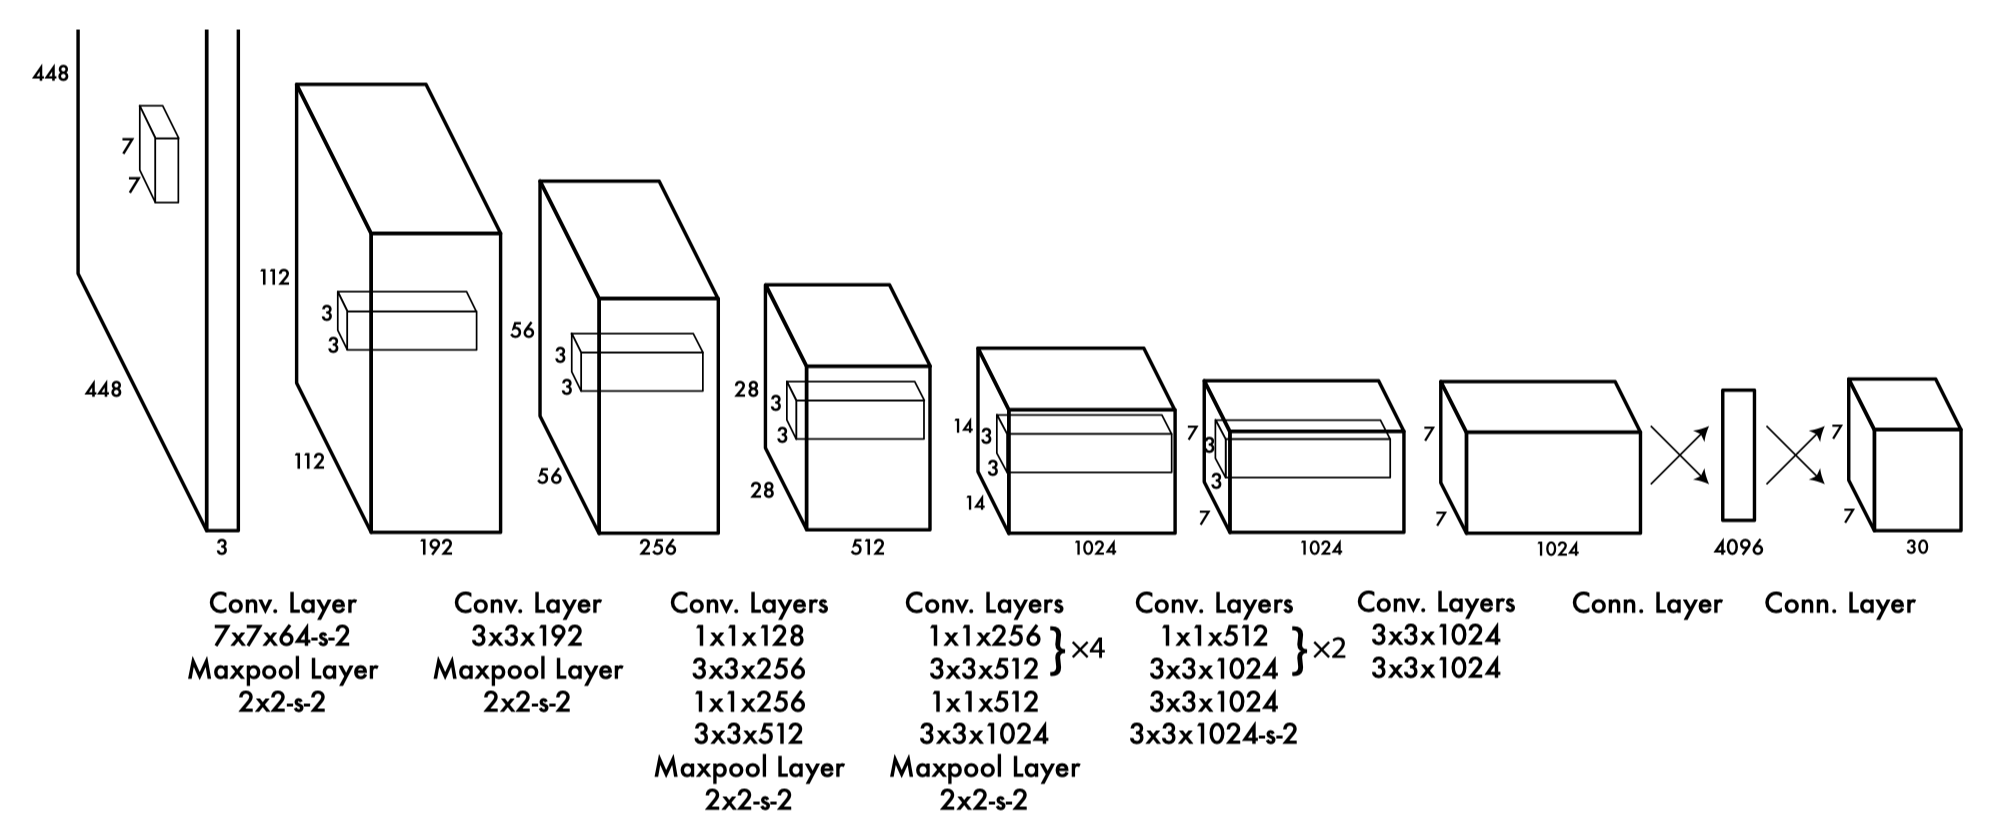
\includegraphics[width=4in]{figures/yolov1_archite.png}
    \caption{YOLOv1 architecture \cite{yolov1_2016}} 
    \label{fig:yolov1_archite}
\end{figure}

The YOLOv1 model is a convolutional neural network (CNN) based on the GoogLeNet model for image classification {\color{red} cite GoogLeNet}. The YOLOv1 model consist of 24 convolutional layer and end with 2 fully connected layer. The overall architecture of YOLOv1 netword is shown in Figure \ref{fig:yolov1_archite}. The author replace the inception layers in GoogLeNet with $1 \times 1$ reduction layer and $3 \times 3$ convolutional layer pair {\color{red} further explain the inception modules and reduction layer}. All the layers in the yolov1 network, with the exception of the final layer, utilize the leaky ReLU activation function {\color{red} cite leaky ReLU}, described as:
\begin{equation*}
    \phi(x) = {\color{red}x if x > 0, 0.1 x otherwise}
\end{equation*}

As we can see in Figure \ref{fig:yolov1_archite}, the last convolutional layers in the network produce a feature map of size $7 \times 7 \times 1024$. This feature map is then processed by two fully connected layers. The last fully connected layer is responsible for predicts both the bounding box and the class label probability \cite{yolov1_2016}. This layer use a linear activation function. The classfication process in the last fully connected layer is simmilar to other CNN where the layer is randomly initialize and can be optimized through training. On the other hand, YOLOv1 proposed a new bounding box regression method that able to  predict all bounding box of all objects present in the image at once, instead of processing each RoI individually one-by-one like the regressor implemented in Faster R-CNN. We will discuss this bouding box generation process in the next subsection.

\subsection{Bounding Box Generation}
To predict bounding box, the YOLOv1 model divide the image into an $S \times S$ grid of equal cells. Each grid cell is then predict $B$ bounding boxes and $C$ probabilities for the $C$ supported classes \cite{yolov1_2016}. The $S$ and $B$ values are hyperparameter and can be fine tune throught experiment. The $C$ value is the number of classes in the training dataset. In other words, $C=20$ if the training dataset is PASCAL VOC \cite{pascal_voc_2015} and $C=80$ if the training dataset is COCO dataset \cite{coco_2014}.

Each bounding box is represented by 5 values: coordinate $x$, coordinate $y$, width $w$, height $h$, and a confidence score. The $(x, y)$ coordinates is the center of the bounding box relative to a grid cell. The width $w$ and height $h$  is the dimension of bouding box in 2D space. The value of $w$ and $h$ are normalized with respect to the input image width and height, thus they are bounded by [0, 1]. The confidence score denote the model confidence in saying there is an object present in this cell, i.e., the objectiveness probability.

\begin{figure}[!ht]
    \centering
    \subfloat[][{\color{red} tobe added}]{ 
        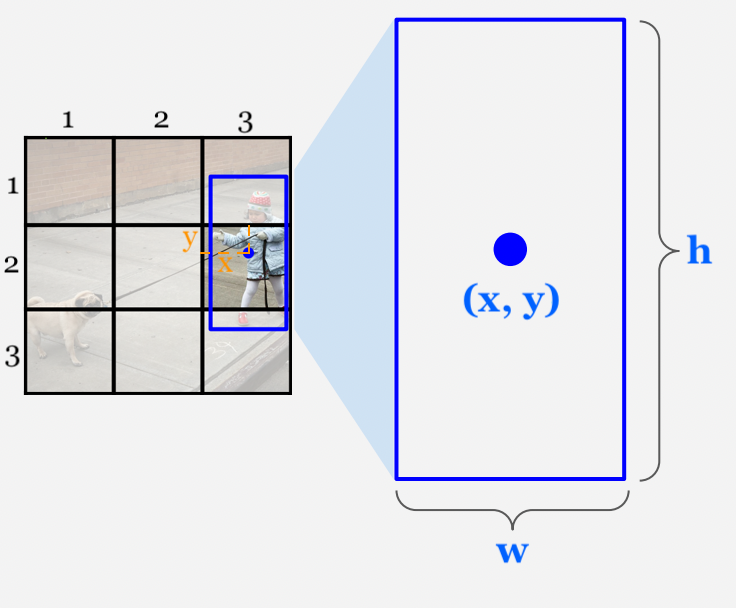
\includegraphics[height=2in]{figures/yolov1_bbox1.png} \label{fig:yolov1_bbox1}
    }
    \qquad \qquad
    \subfloat[][{\color{red} tobe added}]{ 
        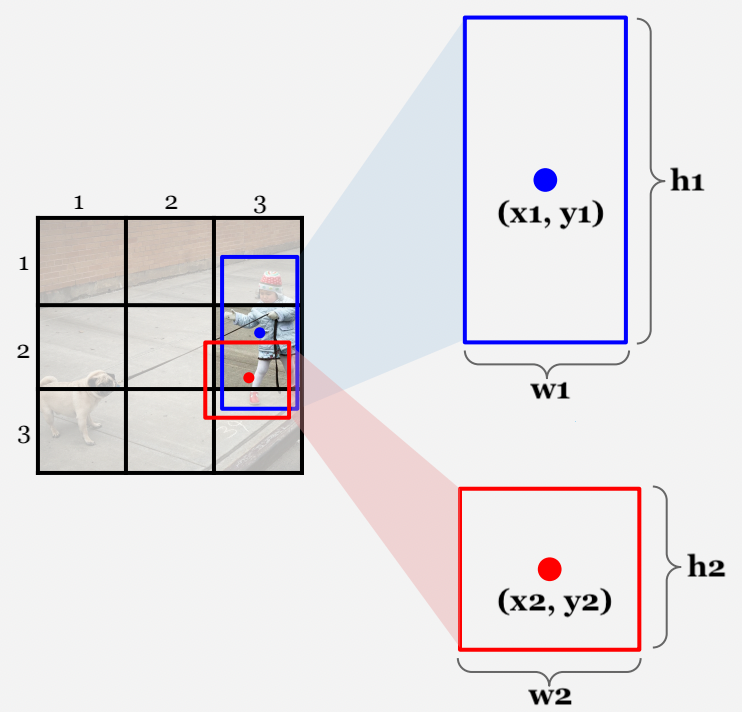
\includegraphics[height=2in]{figures/yolov1_bbox2.png} \label{fig:yolov1_bbox2}
    }
    \caption{{\color{red} tobe added}}
\end{figure}

As an example, consider processing an image with $S=3$, $B=1$, and clasifying between two class human and dog ($C=2$), as demonstrated in Firgure \ref{fig:yolov1_bbox1}. Since $B=1$, which means we only predict one bounding box per cell, then the cell$_{32}$ will return a tensor represent the predicted bounding box as:
\begin{equation*}
    ceil's\ output = \begin{bmatrix}
        {\color{blue} x \quad y \quad w \quad h \quad conf} \quad p_{human} \quad p_{dog}
        \end{bmatrix}
\end{equation*}
where $conf$ is the confidence score, $p_{human}$ and $p_{dog}$ are probability that the object belong to the human and dog class, respectively. Noted that when we only predicting 1 bounding box per ceil, the YOLOv1 model predict $(4+1+2)$ values for each ceil, where 4 value describe the bounding box location, 1 for confidence score, and 2 probality values with one for each class. Therefore we say that when $B=1$, the model predict $(4+1+C)$ for each ceil. 

Now, we consider the example reside in Figure \ref{fig:yolov1_bbox2}, which is the same setup as previous example but with $B=2$. In this second example, we predict two bounding boxes per cell, then the cell$_{32}$ return the following tensor for the two bounding boxes:
\begin{equation*}
    ceil's\ output = \begin{bmatrix}
        {\color{blue} x_1 \quad y_1 \quad w_1 \quad h_1 \quad conf_1} \quad 
        {\color{red} x_2 \quad y_2 \quad w_2 \quad h_2 \quad conf_2} \quad 
        p_{human} \quad p_{dog} 
    \end{bmatrix}
\end{equation*}
The ceil output a $(4+1)*2+C$ elements tensor for when the model predict two bounding boxes per ceil. Therefore, we can generalize the ceil's prediction is encoded as $(4+1)*B+C$ tensor.

The computed prediction for each ceil in the grid is stacked side by side create the depth for the image. That is we divides a 2-dimentional image into a grid of $S \times S$ ceil, we predict a $(4+1)*B+C$ tensor for each ceil, these prediction create the third dimention of the image. Therefore the prediction for the image is encoded as $S \times S \times [(4+1)*B+C]$ tensor. 

The YOLOv1 architecture showned in Figure \ref{fig:yolov1_archite} is for predicting 20 class in PASCAL VOC with $S=7$ and $B=2$, thus the model predicting a $7 \times 7 \times 30$ tensor which encoded multiple bouding boxes and classfication for each ground-truth object. 

\subsection{Training}
The first 20 convolutional layers of YOLOv1 is pretrained with the input size of $224 \times 224$ for classification task on the ImageNet2012 dataset \cite{ImageNet_dataset}. Then four new convolutional layers and 2 fully connected layer are added. These new layers are randomly initialize. Additionally, the input size is increase to $448 \times 448$ for object detection task \cite{yolov1_2016}. With the initialized network, the model generate multiple bounding boxes and classification as described previously. While the YOLOv1 model apply NMS to choose which predicted bounding box to keep at inference time, the author used a different scheme to choose which predicted bounding box to contribute to the loss function. The scheme is choosing the predictor with predicted box that has the highest IoU with a ground truth box. This lead to each predictor have different specilization, which mean each predictor is better at predicting certain size, aspect ratio, or object's class \cite{yolov1_2016}.

The YOLOv1 model is trained to optimize for the sum-square error which encode both the bounding box coordinate loss and the classification loss \cite{yolov1_2016}. While sum-square error allow eazier optimization, it have some shortcomming and not ideal if the model need to optimize for average precision. The first critical shortcomming is the loss weight localization error and classification error equally \cite{yolov1_2016}. In an image, since the majority of the cells does not contain any object, which mean confidence score for these cell are 0, thus cause model always have a poor performance for classification task. This also cause bouding box error to have little affet on the total error. Thus a scalar term is added to the loss to weight the bouding box error higher than the classification error \cite{yolov1_2016}. The second critical shortcomming is sum-squared error weight offset in large bounding box and small bounding box equally \cite{yolov1_2016}. This is not ideal as offset by certain pixels have a larger affect on the smaller bouding box than the larger bounding box, due to total number of pixels in large bounding box is larger than the smaller bounding box. To patially resolve this, the YOLOv1 model perform the error calculation on the squareroot of bounding box width and height instead of the width and height directly.

\section{YOLO9000 (YOLOv2)}  \label{sec:yolov2}

YOLO9000, also known as YOLOv2, is an improvement of the YOLOv1 model \cite{yolo9000_2017}. The real-time object detection model YOLOv2 was first introduced in 2016. The name YOLO9000 stems from the fact that the model is capable of detecting over 9,000 object categories in real time,  which is significantly more than the original YOLO model. This is achieved by finetuning the model with the WordNet language database, which also is the database that the ImageNet labels set pulls from.

\subsection{Accuracy Improvement}
The YOLOv2 model proposes five changes that improve the accuracy of YOLOv1. The first change is the addition of \textbf{batch normalization} on the convolutional layer, which improves the YOLOv1 mAP score by more than 2\%. Batch normalization removes the need for dropout technique \cite{dropout_2014}, which drops certain activated neurons to avoid overfitting problem \cite{szeliski_cv_book}. The second change is utilizing \textbf{higher resolution classifier}. While YOLOv1 only trains on $224 \times 224$ images for the classification task, YOLOv2 further trains the classifier with $448 \times 448$ images. The higher resolution classifier increases the YOLOv1 mAP score by 4\%. The third change is the use of \textbf{passthrough layer}. Since the convolutional layer decreases the image's spatial dimension gradually, thus it becomes more difficult to detect smaller objects in the image as more convolutional layers are used. For this reason, the passthrough layer help brings the image detail from the higher spatial dimension to the lower spatial dimension map, similar to the skip connection in ResNet \cite{resnet_2016}.

Since each divided cell in YOLOv1 only predicts exactly 2 bounding boxes, 1 confidence score, and 1 classification label (the highest probability class), thus the model has poor performance in detecting objects that appear near together, especially small objects. To address this problem, the YOLOv2 model proposes the fourth and fifth changes. 

The fourth change is utilizing \textbf{anchor boxes} at each cell instead of randomly initializing the bounding box like in YOLOv1. The size and aspect ratio of the anchor box heavily depends on the domain that the model will be applied to. For example, when applying the model to the traffic detection task, then the main shape and size the model need to look for are pedestrian and different vehicle. Thus starting the anchor box at these shape and size improve the runtime for both training and inference. For this reason, a k-means clustering algorithm is used to find the top-k common dimension in the training set \cite{yolo9000_2017}. The anchor boxes are then used to predict the bounding box. The YOLOv2 model predicts five parameters for each bounding box $[t_x, t_y, t_w, t_h, and t_o]$, where $t_x, t_y$ and $t_w, t_h$ is the center and the dimension of the bounding box in relation to the cell and the image dimension, respectively. These five parameters are the same as the prediction made by YOLOv1. Given that the cell is $(c_x, x_y)$ offset from the top-left corner of the image, and the anchor box has the dimension of $p_w, p_h$, then the predicted bounding box has the center at $(b_x, b_y)$ with the dimension of $b_w, b_h$, and can be computed with constraint by sigmoid function, as shown in Figure \ref{fig:yolov2_bbox}.

\begin{figure}[!ht]
    \centering
    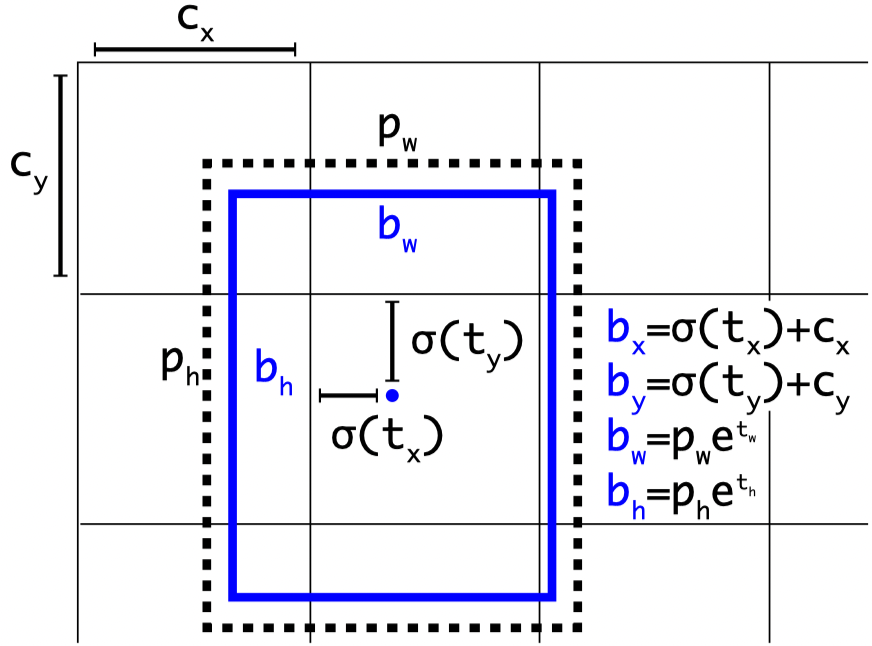
\includegraphics[width=3in]{figures/yolov2_bbox.png}
    \caption{YOLOv2 bounding box (in blue) generation offset from the anchor box (in black) \cite{yolo9000_2017}} 
    \label{fig:yolov2_bbox}
\end{figure}

Since the anchor boxes are used to predict the bounding box, this removes the need for fully connected layers. In addition to the removal of fully connected layers, the YOLOv2 model also moves the classification label from the cell level to the anchor box level. In other words, the YOLOv2 model predicts a classification label for each anchor box \cite{yolo9000_2017}. Let the image be divided into an $S \times S$ cell grid, each cell generates $B$ anchor boxes, and the dataset has $C$ categories, then the image detection is encoded as a $S \times S \times B*(4+1+C)$ tensor. The anchor box scheme removes the assumption of one object per grid cell and improves the mAP score by approximately 5\%.

The fifth change is \textbf{multi-scale training}. Since YOLOv2 remove the fully connected layer, thus it can process images of any size. Therefore, instead of training with a fixed size, the model chooses a new input image dimension every 10 batches. Additionally, since the model is downsampled by 32 times during its process, to avoid quantization, the input image should be a multiple of 32: {320, 352, ..., 608}. This training scheme forces the model to be able to predict object at different resolutions, which train the network to predict object of different scale. In addition to multi-scale training, the model also performs a data augmentation process, including crop, rotation, hue and saturation shift, and exposure shifts to expand the training dataset and further generalize the model.

\subsection{Runtime Improvement}
The YOLOv2 further simplifies the architecture used in YOLOv1. The YOLOv2 model uses a new classification model, namely Darknet-19. The overall architecture of Darknet-19 is shown in Figure \ref{fig:darknet19_archite}. Compared to the GoogLeNet, Darknet-19 is smaller, with 5.58 billion operations instead of 8.52 billion operations, while having higher top-5 accuracy in classification tasks after training \cite{yolo9000_2017}. Compared to YOLOv1's CNN architecture, Darknet-19 only has 19 convolutional layers and 5 max-pooling layers, while YOLOv1's CNN consists of 24 convolutional layers, 4 max-pooling layers, and 2 fully connected layers. The Darknet-19 is first trained with the ImageNet 1000 for the classification task. The Darknet-19 model is then adapted for the object detection task by replacing the last convolutional layer with three $3 \times 3$ convolutional layers that output 1024 channels, followed by $1 \times 1$ convolutional layer to convert $S \times S \times 1024$ to $S \times S \times B*(4+1+C)$.

\begin{figure}[!ht]
    \centering
    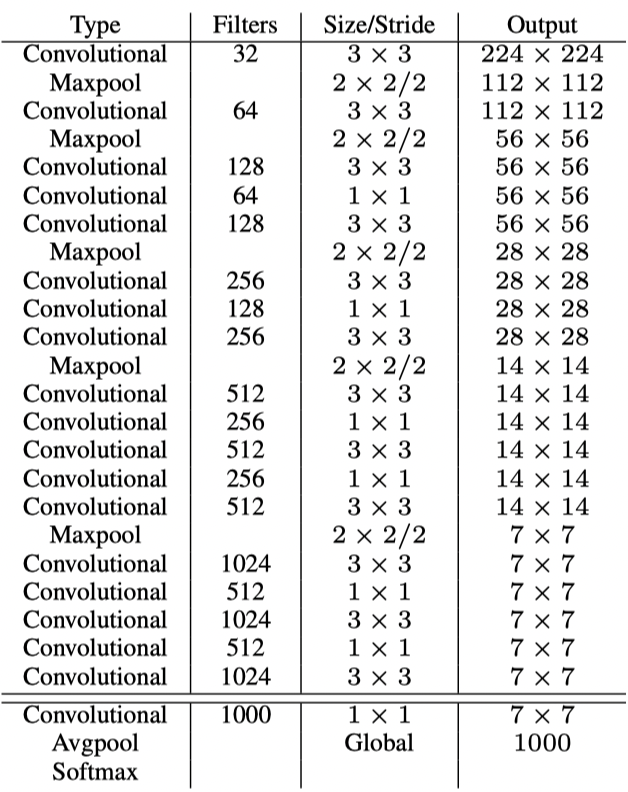
\includegraphics[width=4in]{figures/darknet19_archite.png}
    \caption{Darknet-19 architecture \cite{yolo9000_2017}} 
    \label{fig:darknet19_archite}
\end{figure}

\section{YOLOv3}  \label{sec:yolov3}

The YOLOv3 model is the next incresemental improvement of YOLO family after YOLO9000. The YOLOv3 model is introduced in 2018 \cite{yolov3_2018}, which consist of four main minor changes to YOLOv2 archietecture. 

The first change is replacing the softmax function with independent logistic for the classifier. While the softmax function require the sum of all class's probabilities to 1, independent logistic consider each class independently and the probability of any two class do not affect one another \cite{yolov3_2018}. This improve the model's classifier from multi-class classifier to multi-class and multi-label classifier. That is, when the classifier is multi-class and multi-label, there are no competition between label. For example, if a pedestrian is a women and the supported label include both "pedestrian" and "women", then when use  independent logistic classifier the probability for both label should be high for this object, while softmax classifier will only give high probability to one of the two labels.

While the format of the predicted bounding in YOLOv3 is the same as YOLOv2 (Figure \ref{fig:yolov2_bbox}), the calculation of the confidence score and loss function are different compare to YOLOv2. This is the second change the YOLOv3 proposed compare to YOLOv2. The YOLOv3 predicts the bounding box's confidence (objectness) score is predicted using a logistic regression \cite{yolov3_2018}. This is trained by setting the confidence score of the bounding box anchor to 1 if the anchor box has highest IoU score with the ground-truth box compare to other anchor. During training any anchor box that has IoU score more than 0.5 with a ground-truth box but the IoU score is not the highest among anchor boxes for this object, then that anchor box will not contribute to the loss function. If the model does not predict a bounding box anchor for a ground-truth object, the objectness loss will increase and contribute no affect to localization loss and classification loss. Simmilar to YOLOv1 and YOLOv2, YOLOv3 also optimize for sum-square error loss which combine the localization, classification, and objectness loss into one metric. 

The third change is detection at 3 different scales per cell. At each cell, the model predict $B$ bounding box for each feature map scale i.e., the current feature map and two upscaled feature map. Assume we divide the image into $S \times S$ cells and the dataset is COCO 80 labels, then at each scale the model predict $S \times S \times [3_{bbox} * (4 + 1 + 80)]$, thus the model generate a $S \times N \times [3_{scale} * 3_{bbox} * (4 + 1 + 80)]$ \cite{yolov3_2018}. The YOLOv3 model predict 9 anchor boxes per cell. This 9 anchor boxes is choosen using the k-means clustering algorithm and divided into each scale evenly. For example, the YOLOv3 model trained for COCO dataset will have the following 9 anchor boxes:
\begin{align*}
    Scale-1: &[(10 \times 13), (16 \times 30), (33 \times 23)] \\
    Scale-2: &[(30 \times 61), (62 \times 45), (59 \times 119)] \\
    Scale-3: &[(116  \times  90), (156  \times  198), (373  \times  326)]    
\end{align*}
    
The fourth change is the feature extractor. Inspired by Darknet-19 and ResNet, the author proposed a new CNN archietecture, namely Darknet-53. The overall architechture of Darknet-53 is shown in Firgure \ref{fig:darknet53_archite}.The network consist of 53 convolutional layers, $3 \times 3$ or $1 \times 1$ convolutional layers, and using shortcut connections \cite{yolov3_2018}. The shortcut connections is introduced in ResNet model and is used to skip over certain convolutional layers based on certain conditions, which improve runtime and address problems with high-depth networks \cite{resnet_2016}. The Darknet-53 is two times faster than the ResNet-152 model while perserve the model's accuracy. Other than the loss computation method, the Darknet-53 training is the same as YOLOv2 which include batch normalization, multi-scale training, and data augmentation.
\begin{figure}[!ht]
    \centering
    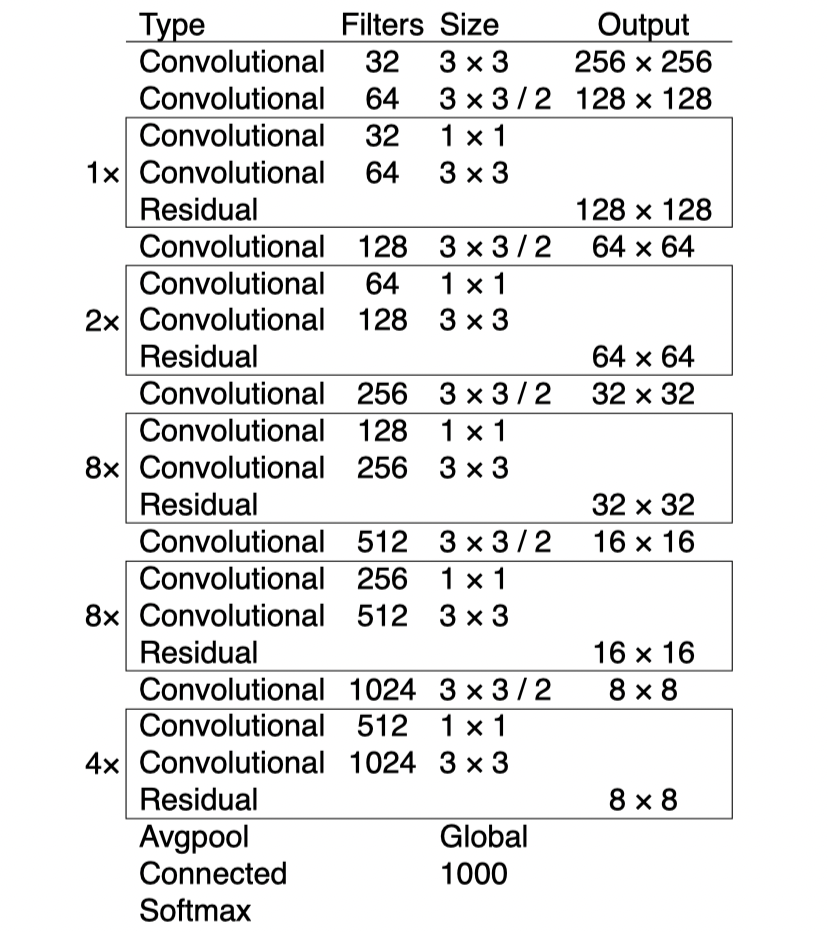
\includegraphics[width=3in]{figures/darknet53_archite.png}
    \caption{Darknet-53 architecture \cite{yolov3_2018}} 
    \label{fig:darknet53_archite}
\end{figure}

\section{YOLOv5}  \label{sec:yolov5}

The YOLOv5 is the fifth entry of the YOLO family. The model is published in 2020 by Ultralytics teams \cite{yolov5_github}. The name YOLOv5 is still controlversal to this date because it is considered as less innovative compare to the YOLOv4 model. While YOLOv4 has a significant change in structure and use some state-of-art algorithm like MISH activation function and GIOU(Generalized Intersection over Union) loss function, YOLOv5 is more focus on ease of use, model size control, and enhancing training data \cite{yolov5_review}. Unfortunately, YOLOv5 model have never had a formal research paper detail explaining the implementation detail, but it has a well documented and supported API developed and maintain by the Ultralytics teams \cite{yolov5_github}. 

At it core, YOLOv5 is YOLOv3 structure with flexible control of model size \cite{yolov5_review}. This is reflected by the API where there are 5 versions of YOLOv5: nano, small, medium, large, and xlarge. Where nano is the smallest version with approximate 12.7 million parameters and xlarge is the largest version with approximate 141.8 million parameters \cite{pytorch_yolov5}. With the different in size, without a doubt, nano version is much faster than the xlarge version at 4.3ms compare to 22.4ms. However, nano version also have a smaller mAP score compare to the xlarge version at 61.9\% compare to 72.0\% on the COCO evaluation set at IoU threshold of 0.5.